\section{Introduction}

Large language models (LLMs) can solve many multi-step problems when prompted to produce a chain of thought (CoT), where intermediate steps are written as natural language tokens before the final answer \cite{paper11}. However, this ties reasoning to the language interface. Language tokens are optimized for communication, not for the core needs of reasoning such as abstraction, conceptualization, and computation. Moreover, autoregressive decoding commits to a single partial trajectory token-by-token, and the compute cost grows linearly with the number of generated tokens \cite{paper14}. These properties make detailed, multi-stage reasoning expensive and brittle: the model must ``think'' by emitting a long, sequential trace.

A large body of work improves CoT reliability using prompting and decoding-time search. Decomposed prompting \cite{paper12}, least-to-most prompting \cite{paper13}, self-consistency and beam-style decoding \cite{paper16}, and tree-based search \cite{paper15} explore or aggregate multiple textual trajectories. Yet they still operate entirely in token space, so they inherit the same sequential bottleneck: each additional unit of reasoning requires more autoregressive tokens. As a result, these methods primarily improve exploration in the same substrate rather than enabling more abstract or information-dense internal computation.

This motivates moving reasoning off the discrete token stream and into the model’s continuous hidden-state space. \emph{Chain of Continuous Thought} (Coconut) replaces spans of textual CoT with continuous latent representations that are never decoded as text and are learned implicitly through their contribution to answer likelihood \cite{paper1}. Coconut shows that latent reasoning can reduce explicit token generation while preserving (and sometimes improving) reasoning behavior.

Why can latent reasoning be more powerful? \emph{Reasoning by Superposition} formalizes an expressivity gap: continuous latent thoughts can represent superpositions of multiple candidate reasoning states within a single step, whereas token-based reasoning must collapse to one discrete path at each decoding step \cite{paper3}. This provides a principled basis for latent reasoning as a mechanism for abstraction and parallel exploration beyond what discrete CoT can represent.

However, existing latent-CoT methods do not fully realize this promise because they remain \emph{autoregressive in latent space}. Coconut generates latent thoughts sequentially by feeding the previous hidden state back as the next input embedding \cite{paper1}. This reintroduces an RNN-like dependency chain inside the Transformer: the critical path length grows linearly with latent depth. Practically, it limits hardware parallelism and makes optimization slower and less stable as we increase latent depth or scale to larger models. More importantly, it constrains \emph{how deeply} latent thinking can be executed in multiple stages, weakening the very benefit latent representations are meant to provide.

Recent work such as \emph{Think Silently, Think Fast} (CoLaR) targets efficiency by compressing token-level reasoning into fewer latent steps and learning the compression policy \cite{paper2}. While effective at shortening trajectories, it retains recurrent latent unrolling and explicitly constrains latents to stay aligned with token-level semantics via reconstruction. As a result, it mainly accelerates reasoning by compressing token-space trajectories, rather than removing the sequential dependency that prevents latent reasoning from scaling to greater depth and model size.

We propose \emph{Codebook Continuous Thought} (CCT), which removes recurrent latent unrolling. Instead of generating latents one-by-one, CCT synthesizes a set of latent thought vectors \emph{in parallel} at each reasoning stage. Concretely, a learnable codebook provides query vectors that cross-attend to the current textual context (and question residual) to produce multiple latent tokens simultaneously (Fig.~\ref{fig:concept_diagram_intro}). These latents then interact bidirectionally within a latent workspace, and the model decodes causally conditioned on the resulting stage latents. Crucially, CCT \emph{re-synthesizes} latents at every stage rather than recursively carrying latent state forward, so reasoning capacity can scale with the number of stages without increasing the serial computation path.

Empirically, CCT matches or exceeds Coconut on mathematical and logical reasoning benchmarks across model scales while reducing training time by 4--9$\times$. Beyond speed, our analyses show that CCT yields more information-rich latent reasoning: (i) fewer latent variables can achieve comparable or better accuracy than recurrent latent unrolling, (ii) increasing latent depth yields consistent gains without requiring increased latent width, and (iii) successive stages encode distinct, context-grounded information rather than redundantly accumulating latent history. Together, these results support the claim that parallel latent synthesis is not only an efficiency trick, but an architectural change that makes continuous latent reasoning more scalable and effective.

\paragraph{Contributions.}
\begin{itemize}
    \item We identify recurrent latent unrolling as the core scaling bottleneck in prior latent-CoT methods: it preserves an autoregressive critical path in latent space, limiting depth, stability, and utilization of hardware parallelism.
    \item We introduce CCT, a stagewise \emph{parallel} latent reasoning mechanism using learnable codebook queries and cross-attention-based synthesis, eliminating recurrent latent dependencies while enabling bidirectional latent deliberation within each stage.
    \item We show that CCT enables scalable latent thinking: it achieves substantial training speedups while matching or improving reasoning accuracy, and it produces more information-dense latent representations that support deeper multi-stage reasoning without increasing latent width.
\end{itemize}

\begin{figure}[h!]
  \centering
  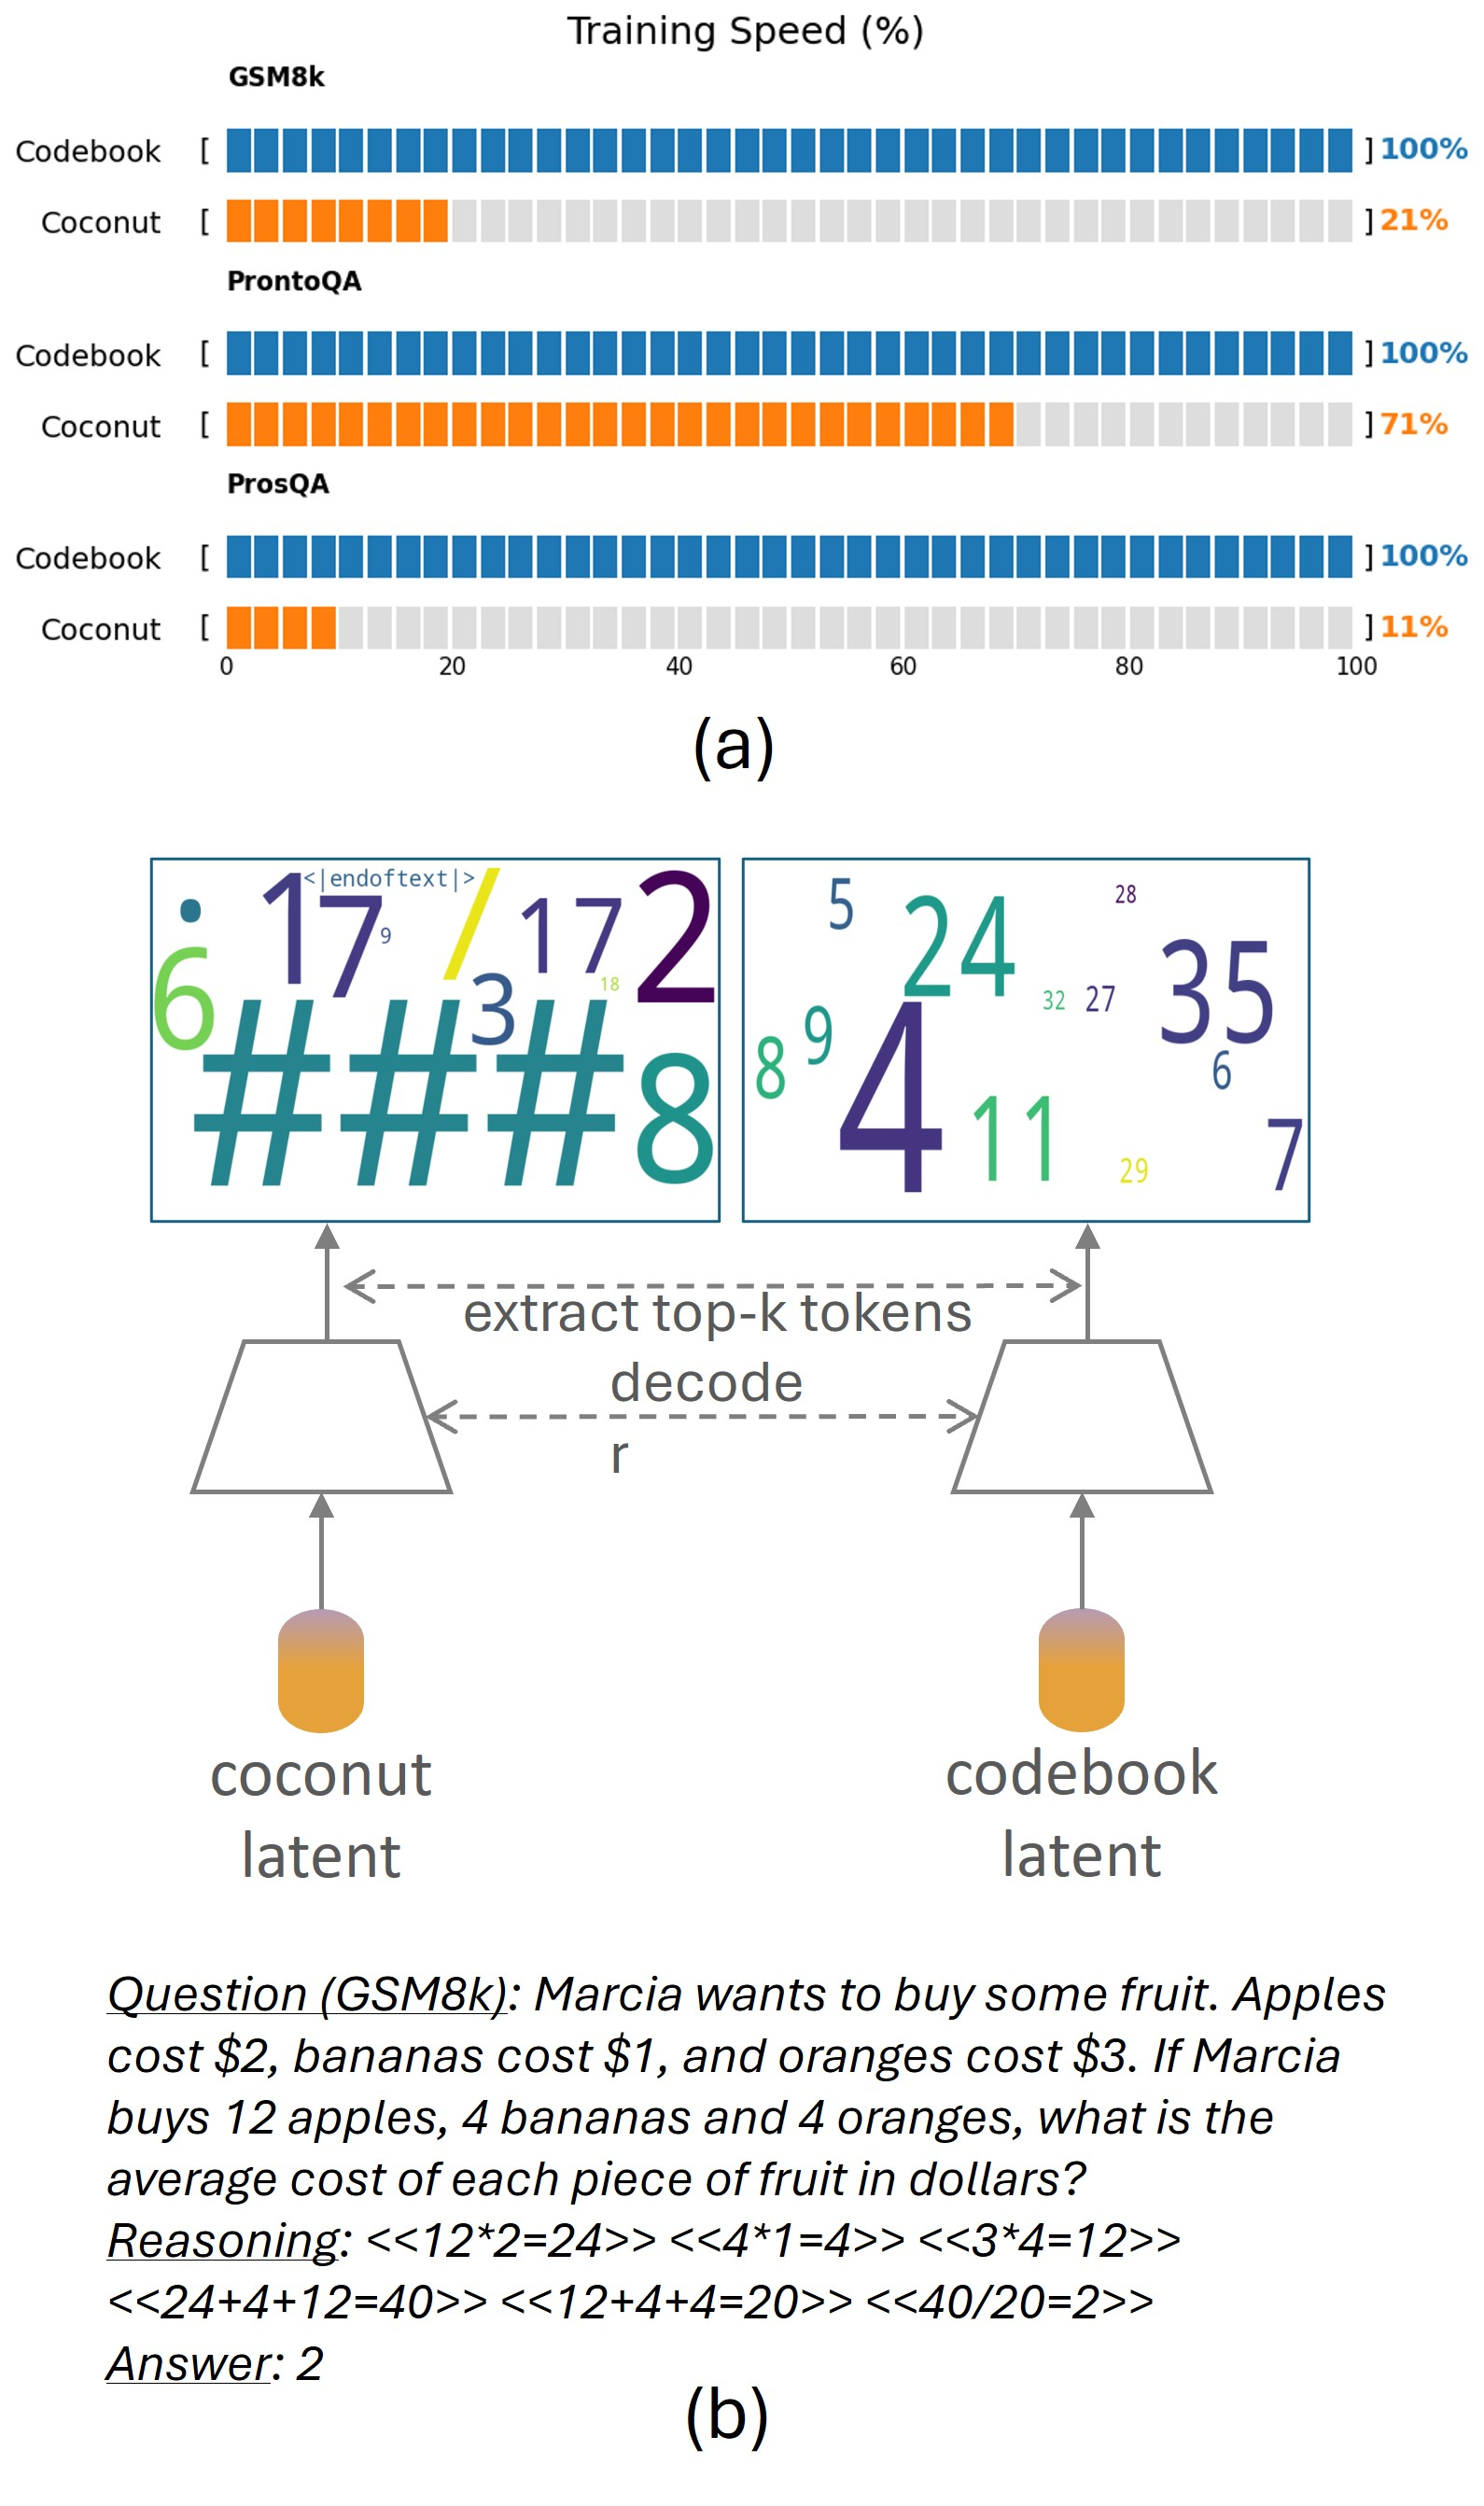
\includegraphics[width=\linewidth]{imgs/concept_diagram_intro.JPG}
  \caption{CCT vs.\ Coconut: (a) training speed and (b) latent quality on GSM8k. Additional examples and latent-to-text probes are provided in the appendix.}
  \label{fig:concept_diagram_intro}
\end{figure}
